\documentclass[]{standalone}
\usepackage{amsmath}
\usepackage{amssymb}
% No page numbers and no paragraph indentation                                  
\pagestyle{empty}                                                               
\setlength{\parindent}{0bp}%
\usepackage{graphicx}
\usepackage{tikz}
\usetikzlibrary{calc,fadings,decorations.pathreplacing,shapes,shapes.multipart,arrows,shapes.misc,intersections,positioning}

\begin{document}

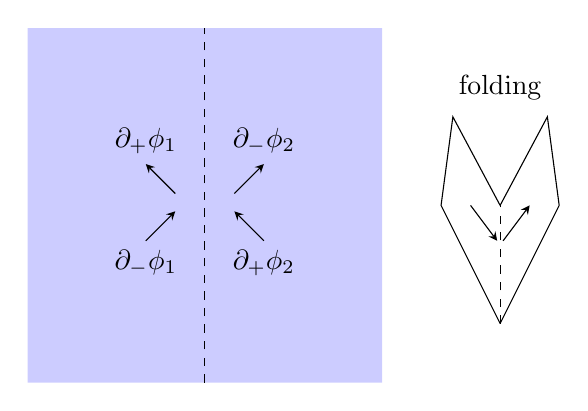
\begin{tikzpicture}[scale = 0.75]
\fill[blue!20] (0,0)--(6,0)--(6,6)--(0,6)--(0,0);
\draw[dashed] (3,0)--++(0,6);
\draw[-stealth] (2,2.4)--++(0.5,0.5);
\draw[-stealth] (2.5,3.2)--++(-0.5,0.5);
\draw[-stealth] (4,2.4)--++(-0.5,0.5);
\draw[-stealth] (3.5,3.2)--++(0.5,0.5);
\node[below] () at (2,2.4) {$\partial_{-} \phi_1$};
\node[above] () at (2,3.7) {$\partial_{+} \phi_1$};
\node[below] () at (4,2.4) {$\partial_{+} \phi_2$};
\node[above] () at (4,3.7) {$\partial_{-} \phi_2$};
\begin{scope}[shift={(8,1)}]
\draw (0,0)--(-1,2)--(-0.8,3.5)--(0,2);
\draw[dashed] (0,0)--(0,2);
\draw (0,0)--(1,2)--(0.8,3.5)--(0,2);
\draw[-stealth] (-0.5,2)--(-0.05,1.4);
\draw[-stealth] (0.05,1.4)--(0.5,2);
\node () at (0,4) {folding};
\end{scope}
\end{tikzpicture}

\end{document}

%%% Local Variables: 
%%% TeX-PDF-mode: t
%%% End: 